\documentclass[../masterarbeit.tex]{subfiles}




\section{Data}

\subsection{Origin of the data}

The avalanche warning service of the energy company VERBUND AG, headquartered in Kaprun, Salzburg, provides the data required to carry out this work. VERBUND represents Austria's leading energy company and is Europe's largest producer of electricity from hydropower. The company states that it obtains almost 100\% of its electricity from renewable sources. The electricity is mainly generated from hydro, wind and photovoltaic power plants. In addition, this is supported by gas-fired thermal power plants \autocites{Verbund:2022}.


The data were recorded in the vicinity of the Mooserboden storage power plant for 39 avalanche strokes. The background for the exceptionally accurate recordings of avalanches is the need for the most accurate possible prediction of avalanches in the 39 avalanche lines around the power plant. Accurate forecasting is of great importance to ensure the safety of the employees working in the areas of the avalanche lines. The power plant is part of the Kaprun power plant group, which includes both pumped and storage power plants. The power plant group is operated by Verbund Hydro Power and is located in Salzburg on the edge of the Hohe Tauern at 2040 meters above sea level and is surrounded by the over 3000 meter high mountains of the Glockner group.\autocites{VerbundKaprun:2022}
 
 


\subsection{Meteorological Data}
 The Data Table Mooser\_Wetter\_Daten includes meteorological data for each day in the months of november to may in the period from 1953 to 2022. The table contains data about the air temperatures at the times 7:00, 14:00 and 19:00 as well as the snow temperature, the wind direction, the wind force, the snow sinking depth, the day weather as well as the weather from the day before, the snow depth, the precipitation, as well as the avalanche degree.

\subsection{Avalanche related data}
The Table Allg\_Lawinen\_Katalog represents general data on all recorded avalanches in the 39 avalanche lines of the area for the same period as the meteorological data from the table Mooser\_Wetter\_Data. More precisely, it contains data such as the type of avalanche, the old ID of the avalanche line where the avalanche went down, the time and date when the avalanche was recorded, the volume of the avalanche, the general weather conditions at the time of the avalanche, as well as general data on the snowpack and the danger level on the day of the avalanche. The Meteorological Data shown in this Table are not used in this study, because the data from the table Mooser\_Wetter\_Daten are homogeneous and available for each day of the winter season. 
Another table of the database named kaplawstr contains additional information about the avalanche lines. For this work, the old and the new code of the avalanche lines are used from this table

\subsection{Topographical Data}
The Topographical Data is recorded in the Database Table TOPP. This table contains several rows for each avalanche line, wich can be identified by the new avalanche line code. The rows record minimum, maximum and mean slope, as well as the orientation and height of the slope. The table also contains various other data columns. These are not used in the further course of the work, since they cannot be assigned to the individual avalanche lines in general, but are connected with individual avalanches, which are not allocated to them in the context of this work. 




\subsection{Data Composition}
 
The database tables Allg\_Lawinen\_Katalog (Avalanche related data), kaplawstr (contains the old as well as the new avalanche line IDs), TOPP (Topographical Data) and Mooser\_Wetter\_Daten (Meteorological data) wich are already described in the previous chapters were merged into a homogeneous data set in the context of this master thesis. This process is explained in detail in this chapter. 
The tables include data from 1944 to 2022. the quality of data increased with the years. This can be shown above all by the fact that in the seasons before 1989/1990 in average, there are 22.0769 per season recorded wich is a lot less than from this season to 2022. In that inteval the average of recorded avalanches is 81.636. This can also be seen in Table 1 wich shows the sum of avalanches recorded per season. With the exception of a few outliers, hardly any avalanches were recorded in these years, and in some cases none at all. In order to increase the homogeneity of the data, all data outside the period from 1989 to 2022 were removed from the database tables.
Subsequently to this measure the kaplawstr table has been merged to the Allg\_Lawinen\_Catalog table using the old avalanche line ID. This adds to each avalanche the associated new avalanche code and avalanche name, which are used as additional ID. The connection is necessary because the TOPP table, which represents the topographic data for the avalanche routes, does not contain the old avalanche route ID. In the course of this step, all lines that were labeled with the avalanche line name "all avalanches" also have been removed. These are not included in the kaplawstr table, since this does not represent an exact departure of an avalanche in one of the avalanche lines, but only states that in many of the avalanche lines small avalanches have departed. 


\begin{table}
    \centering
    \begin{tabular}{|l|l|}
    \hline
        Intervall & Avalanche \\ \hline
        1956/ 1957 & 11 \\ \hline
        1957/ 1958 & 4 \\ \hline
        1958/ 1959 & 7 \\ \hline
        1959/ 1960 & 62 \\ \hline
        1964/ 1965 & 8 \\ \hline
        1965/ 1966 & 8 \\ \hline
        1966/ 1967 & 15 \\ \hline
        1967/ 1968 & 9 \\ \hline
        1968/ 1969 & 3 \\ \hline
        1969/ 1970 & 20 \\ \hline
        1970/ 1971 & 22 \\ \hline
        1971/ 1972 & 0 \\ \hline
        1972/ 1973 & 67 \\ \hline
        1973/ 1974 & 31 \\ \hline
        1974/ 1975 & 78 \\ \hline
        1976/ 1977 & 0 \\ \hline
        1979/ 1980 & 27 \\ \hline
        1980/ 1981 & 40 \\ \hline
        1981/ 1982 & 29 \\ \hline
        1982/ 1983 & 27 \\ \hline
        1983/ 1984 & 0 \\ \hline
        1984/ 1985 & 10 \\ \hline
        1985/ 1986 & 24 \\ \hline
        1986/ 1987 & 37 \\ \hline
        1987/ 1988 & 17 \\ \hline
        1988/ 1989 & 18 \\ \hline
        1989/ 1990 & 66 \\ \hline
        1990/ 1991 & 55 \\ \hline
        1991/ 1992 & 133 \\ \hline
        \end{tabular}
        \begin{tabular}{|l|l|}
        \hline
        Intervall & Avalanche \\ \hline
        1992/ 1993 & 80 \\ \hline
        1993/ 1994 & 47 \\ \hline
        1994/ 1995 & 93 \\ \hline
        1995/ 1996 & 3 \\ \hline
        1996/ 1997 & 19 \\ \hline
        1997/ 1998 & 18 \\ \hline
        1998/ 1999 & 90 \\ \hline
        1999/ 2000 & 128 \\ \hline
        2000/ 2001 & 89 \\ \hline
        2001/ 2002 & 124 \\ \hline
        2002/ 2003 & 84 \\ \hline
        2003/ 2004 & 92 \\ \hline
        2004/ 2005 & 97 \\ \hline
        2005/ 2006 & 100 \\ \hline
        2006/ 2007 & 40 \\ \hline
        2007/ 2008 & 86 \\ \hline
        2008/ 2009 & 79 \\ \hline
        2009/ 2010 & 52 \\ \hline
        2010/ 2011 & 52 \\ \hline
        2011/ 2012 & 150 \\ \hline
        2012/ 2013 & 121 \\ \hline
        2013/ 2014 & 55 \\ \hline
        2014/ 2015 & 75 \\ \hline
        2015/ 2016 & 66 \\ \hline
        2016/ 2017 & 67 \\ \hline
        2017/ 2018 & 133 \\ \hline
        2018/ 2019 & 177 \\ \hline
        2019/ 2020 & 67 \\ \hline
        2020/ 2021 & 130 \\ \hline
        2021/ 2022 & 26 \\ \hline
    \end{tabular}
    \caption{recorded Avalanches per Season}
\end{table}



\begin{lstlisting}[language=Python, caption=calculation of TOPP data for every avalanche line]
TOPP = kaplawstr['Code_neu'].apply(lambda x: TOPP.loc[TOPP['Lawinencode'] == x].mean())
\end{lstlisting} 
In the second step, the average values for all columns from the associated avalanches were calculated from the TOPP table for each avalanche line. The python code shown in Listing 1 demonstrates this process. By this measure, one row is created for each avalanche line. The table contained without this procedure a total of 1905 rows. In the default state, the table could not have been connected to the other data tables. Another way to get only one row per avalanche stroke would be to select a random value for the respective stroke. The reason for taking the average value is that there are not the same number of lines for all avalanche lines and the values of the individual lines per avalanche line do not differ greatly from each other. Thus, the average value represents the entirety of the lines per stroke consistently. The topographic data from the newly assembled TOPP table was then merged to the entire dataset using the new avalanche ID. \newline
Subsequently, these avalanches were assigned to the daily recorded meteorological data of the Mooser\_Wetter\_Data table by an outer join, so as result there is at least one row per day in the dataset. In cases where several large avalanches have occurred at the same day, the dataset contains one row per avalanche and each Includes the meteorological data for this day. \newline \newline
In order to train a machine learning algorithm for the prediction of avalanches for topographically defined slopes in conjunction with the meteorological data available for this work, the topographical data must also be mapped onto the days without avalanches. The algorithm needs this information, as the data set would otherwise only contain topographic data directly related to avalanches. This would mean, for example, that the slope inclination could not become a feature for the prediction.
\\
\begin{lstlisting}[language=Python, caption=mapping random sample lines of topographical data onto the rows of non avalanche days]
for i in gesamt_df.index:
    if(pd.isnull(gesamt_df['meanExpo'][i])):
        sample = TOPP.sample(1)
        gesamt_df['meanExpo'][i] = sample['meanExpo'].values[0]
        gesamt_df['meanSlope'][i] = sample['meanSlope'].values[0]
        gesamt_df['stdDevSlope'][i] = sample['stdDevSlope'].values[0]
        gesamt_df['MinSlope'][i] = sample['MinSlope'].values[0]
        gesamt_df['MaxSlope'][i] = sample['MaxSlope'].values[0]
        gesamt_df['Altitude'][i] = sample['Altitude'].values[0]
\end{lstlisting} 
The consequence of this is that the topographic data must also be mapped to the days without avalanches. Because these days are not connected to an avalanche line ID and an even distribution on the slopes on these days is required, random lines from the calculated mean values of the TOPP table were mapped to them. Listing 2 shows this process in form of the corresponding Python code.
The resulting dataset maps 7055 rows and 139 columns. 2728 of these rows are recorded avalanches departures. The dataset contains columns that are redundant, empty, sparsely filled or contain information wich can not be used to train a machine learning algorithm. Figure 2 shows a heatmap of the Nan values in the dataset. As mentioned in chapter 3.1 about feature selection, these columns have a huge cost in computation time, decrease the prediction performance and increase the error rate. This requires the measure to remove all columns with these characteristics.
\\
\begin{figure}[h]
    \centering
    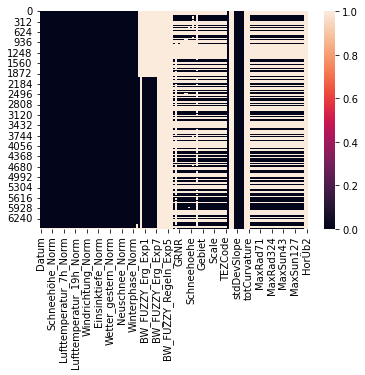
\includegraphics[scale=1.0]{heatmap_nanValues.png}
    \caption{Heatmap to show the distribution of Nan values in the dataset}
\end{figure}
\\
After dropping this features the Dataset includes 46 columns. 
In addition, a new column was added to the dataset, which contains either a 1 in case of an avalanche or a 0 in case no avalanche has occurred. This column is added to make it possible to predict  whether an avalanche will occur or not. To train a machine learning algorithm on predicting whether an avalanche will go down from a particular slope, all features that can be used to directly and without any other features determine whether an avalanche will descend must be removed from the dataset.




